\section{Potenzfunktionen}
\subsection{Definition}
Betrachtet man eine Funktion $f(x)=x^n$, wobei $n\in\setminus\{0\}$, so spricht man von einer Potenzfunktion. Der Begriff `{}Potenzfunktion`{} ist hierbei ein Schirmbegriff für alle Funktionen, die eine Potenz besitzen. Im Folgenden unterscheidet man zwischen
\begin{itemize}
	\item $n>0 \land n\equiv0(mod2)$ Bedeutet, dass $n$ größer als 0 ist und einen kongruenten Modulo hat für den Modulo aus 2 und den Wert $0$. Wird $n$ geteilt durch $2$, so muss der Modulo $0$ ergeben.
	\item $n>0$ und $ n\equiv1(mod2)$
	\item $n<0$ und $ n\equiv0(mod2)$
	\item $n<0$ und $ n\equiv1(mod2)$
\end{itemize}
\subsection{Potentfunktion mit $n>0 $ und $ n\equiv0(mod2)$}
Ist $n$ gerade und positiv, so hat eine Funktion $f(x)=x	^n$ folgende Eigenschaften.
\begin{itemize}
	\item Der Graph ist Achsensymmetrisch zu der $Y$-Achse
	\item Der Graph verläuft parabolisch
	\item Für $x<0$ steigt der Graph
	\item Für $x>0$ steigt der Graph
	\item Je höher der Exponent, desto flacher verläuft der Graph für $-1<x>1$ und desto steiler für $x>1$ und $x<-1$
\end{itemize}
\begin{figure}[h!]
\centering
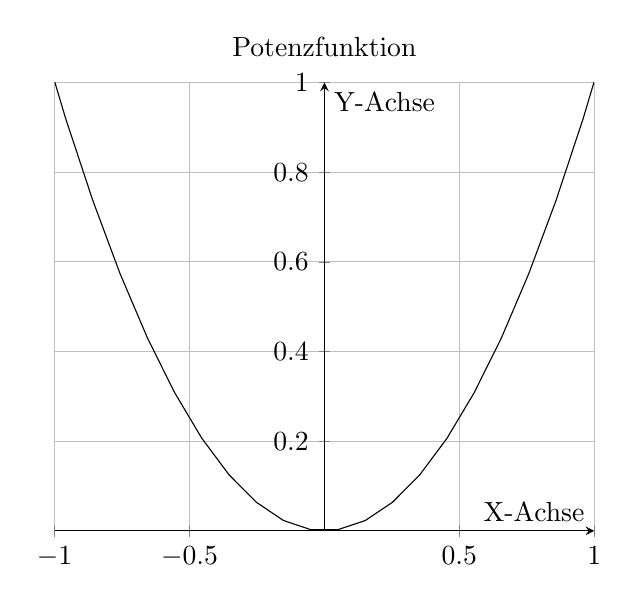
\begin{tikzpicture}
\begin{axis}[
    title={Potenzfunktion},
    xlabel={X-Achse},
    ylabel={Y-Achse},
    axis lines=middle, % Zentriert die Achsen
    xmin=-1, xmax=1, % Setzt die Grenzen für die X-Achse
    ymin=0, ymax=1, % Setzt die Grenzen für die Y-Achse
    grid=major, % Fügt ein Hauptgitter hinzu
]
\addplot[mark=none, samples=100] {x^2};
\end{axis}
\end{tikzpicture}
\caption{Quadratische Funktion mit $n>0$ und $ n\equiv0(mod2)$}
\end{figure}
\geogebra{https://www.geogebra.org/m/cand2jpf}
\subsection{Potenzfunktion mit $n>0$ und $ n\equiv1(mod2)$}
Ist $n>0$ und ungerade, so hat $f(x)=x^n$ die folgenden Eigenschaften.
\begin{itemize}
	\item $f(x)$ ist punktsymmetrisch zum Ursprung
	\item $f(x)$ verläuft von links nach rechts (vom 1. Quadranten zum 3. Quadranten), dies bedeutet die Form ist kubisch. %TODO Quadranten Blatt hinzufügen
	\item Je größer der Exponent ist, desto flacher verläuft $f$ für $-1<x<1$ und steiler für $x>1$ bzw. $x<-1$
	\item Die Funktion, die die geben Eigenschaften erfüllen sind alle monoton steigend
\end{itemize}
\begin{figure}[h!]
\centering
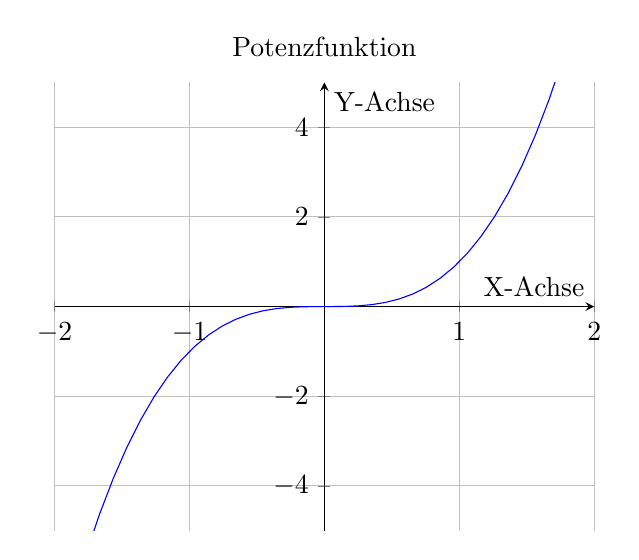
\begin{tikzpicture}
\begin{axis}[
    title={Potenzfunktion},
    xlabel={X-Achse},
    ylabel={Y-Achse},
    axis lines=middle, % Zentriert die Achsen
    xmin=-2, xmax=2, % Setzt die Grenzen für die X-Achse
    ymin=-5, ymax=5, % Setzt die Grenzen für die Y-Achse
    grid=major, % Fügt ein Hauptgitter hinzu
]
\addplot+[mark=none, samples=100]{x^3};
\end{axis}
\end{tikzpicture}
\caption{Potenzfunktion mit $n>0$ und $ n\equiv1(mod2)$}
\end{figure}
\subsection{Potenzfunktion mit $n<0$ und $ n\equiv0(mod2)$ - Hyperbel}
Hat eine Funktion $f(x)=x^n$ einen negativen Exponenten, so bezeichnet man die Funktion als Hyperbel. Hyperbeln haben eine Definitionslücke, dass heißt, es gibt Zahlen, die man nicht für $x$ einsetzten darf. Hyperbeln verlaufen asymptotisch, dass heißt, es existieren Geraden, deren sich der Graph unendlich nah annähert, diese allerdings nicht tangiert. Besitzen sie einen geraden Exponenten verlaufen sie Achsensymmetrisch. Ist der Exponent ungerade, so verläuft der Graph Punktsymmetrisch. 
\begin{figure}[h!]
\centering
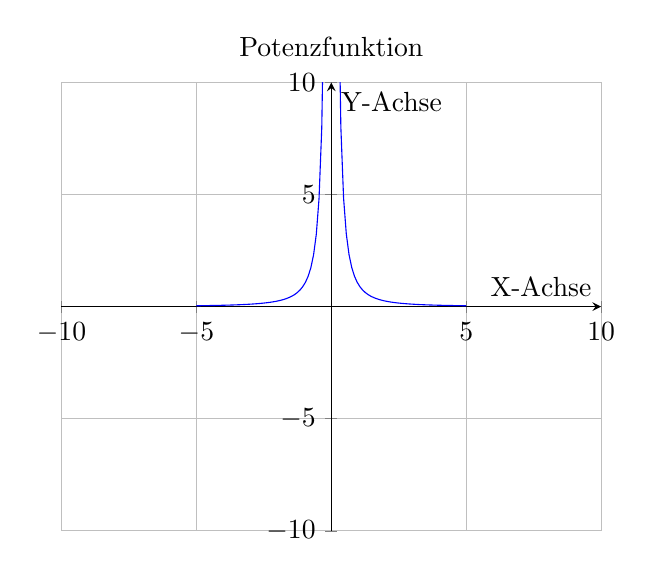
\begin{tikzpicture}
\begin{axis}[
    title={Potenzfunktion},
    xlabel={X-Achse},
    ylabel={Y-Achse},
    axis lines=middle, % Zentriert die Achsen
    xmin=-10, xmax=10, % Setzt die Grenzen für die X-Achse
    ymin=-10, ymax=10, % Setzt die Grenzen für die Y-Achse
    grid=major, % Fügt ein Hauptgitter hinzu
]
\addplot+[mark=none, samples=100]{x^(-2)};
\end{axis}
\end{tikzpicture}
\caption{Potenzfunktion mit $n<0$ und $ n\equiv0(mod2)$}
\label{}
\end{figure}

